\documentclass[zihao=5,a4paper,UTF8]{ctexart}
\usepackage[top=2.0cm, bottom=2.0cm, left=2.0cm, right=2.0cm]{geometry}
\usepackage{amsmath, amssymb, bm}
\newcommand{\vect}[1]{\bm{#1}}
\newcommand{\ee}{\mathrm{e}}
\usepackage{array, booktabs}
\usepackage{enumitem}
\usepackage{tikz}
\usepackage{fancyhdr}

\pagestyle{fancy}
\fancyhf{}
\fancyfoot[C]{\small 第 \thepage\ 页}
\renewcommand{\headrulewidth}{0pt}

\newcommand{\blank}[1][2.5cm]{\underline{\hspace{#1}}}
\newcommand{\choicebox}{\hfill(\hspace{1.8em})}

\begin{document}

\begin{center}
    {\Large\bfseries 南京航空航天大学}\\[4pt]
    {\large 2022 $\sim$ 2023 学年\ 第 1 学期\ 《大学物理 I(2)》、《大学物理 IA(2)》考试试题}
\end{center}

\begin{center}
\begin{tabular}{|c|c|c|c|c|}
\hline
题号 & 一（36分） & 二（30分） & 三（34分） & 总分 \\
\hline
得分 & \hspace{2.2cm} & \hspace{2.2cm} & \hspace{2.2cm} & \hspace{2.2cm} \\
\hline
\end{tabular}
\end{center}

\section*{一、选择题（每小题 3 分，共 36 分）}

\begin{enumerate}[leftmargin=2em, itemsep=6pt]
    \item 一个质点作简谐运动，振幅为 $A$，在起始时刻质点的位移为 $A/2$，且向 $x$ 轴负方向运动，代表此简谐运动的旋转矢量图为：\choicebox\\
    \begin{center}
    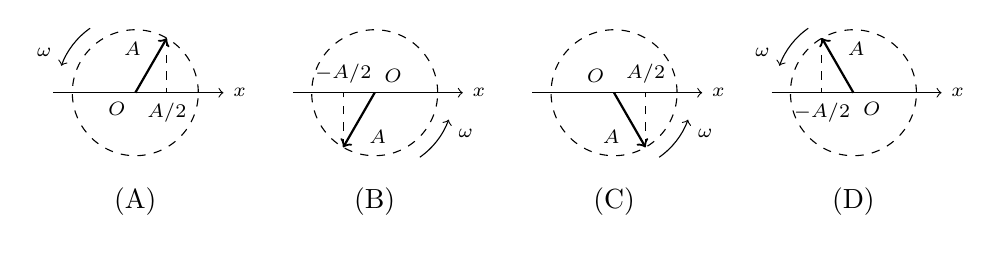
\begin{tikzpicture}[scale=0.80]
        % (A)
        \begin{scope}
            \draw[dashed] (0,0) circle (1);
            \draw[->] (-1.3,0) -- (1.4,0) node[right] {\scriptsize $x$};
            \draw[->, thick] (0,0) -- (60:1) node[midway, above left] {\scriptsize $A$};
            \draw[dashed] (60:1) -- (0.5,0) node[below] {\scriptsize $A/2$};
            \node[below left] at (0,0) {\scriptsize $O$};
            \draw[->] (125:1.25) arc (125:160:1.25) node[above left] {\scriptsize $\omega$};
            \node[below] at (0,-1.35) {(A)};
        \end{scope}
        % (B)
        \begin{scope}[xshift=3.8cm]
            \draw[dashed] (0,0) circle (1);
            \draw[->] (-1.3,0) -- (1.4,0) node[right] {\scriptsize $x$};
            \draw[->, thick] (0,0) -- (-120:1) node[midway, below right] {\scriptsize $A$};
            \draw[dashed] (-120:1) -- (-0.5,0) node[above] {\scriptsize $-A/2$};
            \node[above right] at (0,0) {\scriptsize $O$};
            \draw[->] (-55:1.25) arc (-55:-20:1.25) node[below right] {\scriptsize $\omega$};
            \node[below] at (0,-1.35) {(B)};
        \end{scope}
        % (C)
        \begin{scope}[xshift=7.6cm]
            \draw[dashed] (0,0) circle (1);
            \draw[->] (-1.3,0) -- (1.4,0) node[right] {\scriptsize $x$};
            \draw[->, thick] (0,0) -- (-60:1) node[midway, below left] {\scriptsize $A$};
            \draw[dashed] (-60:1) -- (0.5,0) node[above] {\scriptsize $A/2$};
            \node[above left] at (0,0) {\scriptsize $O$};
            \draw[->] (-55:1.25) arc (-55:-20:1.25) node[below right] {\scriptsize $\omega$};
            \node[below] at (0,-1.35) {(C)};
        \end{scope}
        % (D)
        \begin{scope}[xshift=11.4cm]
            \draw[dashed] (0,0) circle (1);
            \draw[->] (-1.3,0) -- (1.4,0) node[right] {\scriptsize $x$};
            \draw[->, thick] (0,0) -- (120:1) node[midway, above right] {\scriptsize $A$};
            \draw[dashed] (120:1) -- (-0.5,0) node[below] {\scriptsize $-A/2$};
            \node[below right] at (0,0) {\scriptsize $O$};
            \draw[->] (125:1.25) arc (125:160:1.25) node[above left] {\scriptsize $\omega$};
            \node[below] at (0,-1.35) {(D)};
        \end{scope}
    \end{tikzpicture}
    \end{center}

    \item 如图，一个球冠形光滑凹槽深度 $h=0.050\ \mathrm{m}$，球半径为 $20\ \mathrm{m}$。现将一质量为 $0.10\ \mathrm{kg}$ 的小球放在凹槽边缘从静止释放。重力加速度大小为 $9.8\ \mathrm{m/s^2}$。小球由凹槽最高点滑到最低点所用时间为\choicebox\\
    \begin{minipage}[t]{0.66\textwidth}
    (A) $2.24\ \mathrm{s}$\qquad (B) $1.12\ \mathrm{s}$\qquad (C) $2\ \mathrm{s}$\qquad (D) $1\ \mathrm{s}$
    \end{minipage}%
    \begin{minipage}[t]{0.32\textwidth}
    \centering
    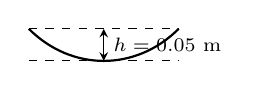
\begin{tikzpicture}[scale=0.68, baseline=(current bounding box.north)]
        \draw[thick] (-1.4,0.6) .. controls (-0.6,-0.2) and (0.6,-0.2) .. (1.4,0.6);
        \draw[dashed] (-1.4,0.6) -- (1.4,0.6);
        \draw[dashed] (-1.4,0.0) -- (1.4,0.0);
        \draw[<->, >=stealth] (0,0.0) -- (0,0.6) node[midway, right] {\scriptsize $h=0.05\ \mathrm{m}$};
    \end{tikzpicture}
    \end{minipage}

    \item 下图（a）表示沿 $x$ 轴正向传播的平面简谐波在 $t=0$ 时刻的波形图，则图（b）表示的是：\choicebox\\
    \begin{minipage}[t]{0.46\textwidth}
    (A) 质点 $m$ 的振动曲线；\qquad (B) 质点 $n$ 的振动曲线；\\
    (C) 质点 $p$ 的振动曲线；\qquad (D) 质点 $q$ 的振动曲线。
    \end{minipage}%
    \begin{minipage}[t]{0.52\textwidth}
    \centering
    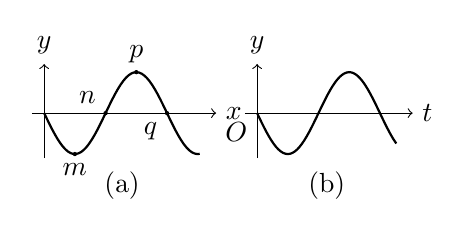
\begin{tikzpicture}[scale=0.52, baseline=(current bounding box.north)]
        % (a)
        \draw[->] (-0.3,0) -- (4.2,0) node[right] {$x$};
        \draw[->] (0,-1.1) -- (0,1.2) node[above] {$y$};
        \draw[thick, domain=0:3.8, samples=60] plot (\x, {-sin(120*\x)});
        \fill (0.75,-1) circle (1.5pt) node[below] {$m$};
        \fill (1.5,0) circle (1.5pt) node[above left] {$n$};
        \fill (2.25,1) circle (1.5pt) node[above] {$p$};
        \fill (3.0,0) circle (1.5pt) node[below left] {$q$};
        \node[below] at (1.9,-1.2) {(a)};
        % (b)
        \begin{scope}[xshift=5.2cm]
            \draw[->] (-0.3,0) -- (3.8,0) node[right] {$t$};
            \draw[->] (0,-1.1) -- (0,1.2) node[above] {$y$};
            \draw[thick, domain=0:3.4, samples=60] plot (\x, {-sin(120*\x)});
            \node[below left] at (0,0) {$O$};
            \node[below] at (1.7,-1.2) {(b)};
        \end{scope}
    \end{tikzpicture}
    \end{minipage}

    \item 一平面谐波，频率为 $100\ \mathrm{Hz}$，波速 $360\ \mathrm{m/s}$，在波线上有 $A$、$B$ 两点，相位差为 $\varphi_A - \varphi_B = -\pi/3$，则两点的距离为\choicebox\\
    (A) $0.6\ \mathrm{m}$，且 $A$ 点距波源较近；\qquad (B) $1.2\ \mathrm{m}$，且 $A$ 点距波源较近；\\
    (C) $0.6\ \mathrm{m}$，且 $B$ 点距波源较近；\qquad (D) $1.2\ \mathrm{m}$，且 $B$ 点距波源较近。

    \item 玻璃上均匀镀有一层介质薄膜，其折射率 $n$ 大于玻璃的折射率，假定光线垂直照射玻璃，要使得某一波长 $\lambda$ 透射光增强，则介质膜的最小厚度应为\choicebox\\
    (A) $\frac{\lambda}{n}$\qquad (B) $\frac{\lambda}{2n}$\qquad (C) $\frac{\lambda}{3n}$\qquad (D) $\frac{\lambda}{4n}$

    \item 波长 $\lambda = 5000\ \text{\AA}$ 的单色光垂直照射到宽度 $a=0.25\ \mathrm{mm}$ 的单缝上，单缝后面放置一凸透镜，在凸透镜的焦平面上放置一屏幕，用以观测衍射条纹，今测得屏幕上中央明条纹一侧第三个暗条纹和另一侧第三个暗条纹之间的距离 $d=12\ \mathrm{mm}$，则凸透镜的焦距 $f$ 为：\choicebox\\
    (A) $2\ \mathrm{m}$\qquad (B) $0.2\ \mathrm{m}$\qquad (C) $0.5\ \mathrm{m}$\qquad (D) $1\ \mathrm{m}$\qquad (E) $0.1\ \mathrm{m}$

    \item 双缝衍射实验，若保持双缝 $S_1$ 和 $S_2$ 的中心之间的距离不变，把两条缝的宽度 $a$ 逐渐加宽，则\choicebox\\
    (A) 单缝衍射的中央明纹区变宽，其中包含的干涉条纹的数目变少；\\
    (B) 单缝衍射的中央明纹区变窄，其中包含的干涉条纹的数目不变；\\
    (C) 单缝衍射的中央明纹区变窄，其中包含的干涉条纹的数目变多；\\
    (D) 单缝衍射的中央明纹区变窄，其中包含的干涉条纹的数目变少。

    \item 使光强为 $I_0$ 的平面偏振光先后通过两个偏振片 $P_1$ 和 $P_2$，$P_1$ 和 $P_2$ 的偏振化方向与原入射光矢量振动方向的夹角分别是 $\alpha$ 和 $90^\circ$，$\alpha$ 为锐角，则通过这两个偏振片后的光强 $I$ 是\choicebox\\
    (A) $\frac{1}{2}I_0\cos^2\alpha$\qquad (B) $0$\qquad (C) $\frac{1}{4}I_0\sin^2(2\alpha)$\qquad (D) $\frac{1}{4}I_0\sin^2\alpha$

    \item 波长 $\lambda=5000\ \text{\AA}$ 的光波沿 $x$ 轴正向传播，若光的波长的不确定量 $\Delta\lambda = 10^{-3}\ \text{\AA}$，则利用不确定关系式 $\Delta p_x \Delta x \ge h$ 可得光子的 $x$ 坐标的不确定量至少为：\choicebox\\
    (A) $25\ \mathrm{cm}$\qquad (B) $50\ \mathrm{cm}$\qquad (C) $250\ \mathrm{cm}$\qquad (D) $500\ \mathrm{cm}$

    \item 已知粒子处于宽度为 $a$ 的一维无限深势阱中的波函数为 $\psi_n(x) = A\sin\frac{n\pi x}{a}\ee^{-\frac{\mathrm{i}}{\hbar}E_n t}\ (n=1,2,3,\dots)$，则当 $n=1$ 基态时，在 $x_1=0 \to x_2=a/3$ 区间粒子出现的概率为\choicebox\\
    (A) $0.098$\qquad (B) $0.196$\qquad (C) $0.333$\qquad (D) $0.804$

    \item 在均匀磁场 $B$ 内放置一极薄的金属片，其产生光电效应的红限波长为 $\lambda_0$。今用单色光照射，发现有光电子逸出，有些放出的光电子（质量为 $m$，电荷的绝对值为 $e$）在垂直于磁场的平面内作半径为 $R$ 的圆周运动，那么此照射光的光子能量是（不考虑相对论效应）\choicebox\\
    (A) $\frac{hc}{\lambda_0} + \frac{(eRB)^2}{2m}$\qquad (B) $\frac{hc}{\lambda_0}$\qquad (C) $\frac{hc}{\lambda_0} + \frac{eRB}{m}$\qquad (D) $\frac{hc}{\lambda_0} + 2eRB$

    \item 某金属产生光电效应的红限频率为 $\nu_0$，当用频率为 $\nu\ (\nu > \nu_0)$ 的单色光照射该金属时，从金属中逸出的光电子（质量为 $m$）的德布罗意波长为（不考虑相对论效应）\choicebox\\
    (A) $\sqrt{\frac{h}{2m(\nu+\nu_0)}}$\qquad (B) $\sqrt{\frac{h}{2m(\nu-\nu_0)}}$\qquad (C) $\sqrt{\frac{h\nu_0}{2m\nu}}$\qquad (D) $\sqrt{\frac{2h}{m(\nu-\nu_0)}}$
\end{enumerate}

\section*{二、填空题（每空 3 分，共 30 分）}

\begin{enumerate}[leftmargin=2em, itemsep=6pt, start=13]
    \item \begin{minipage}[t]{0.66\textwidth}
    水平静止的车厢中，用一根劲度系数为 $k$ 的轻弹簧水平连接质量为 $m$ 的小滑块，弹簧无伸长，滑块静止，滑块与车厢底板间无摩擦。如图所示，现使车厢以恒定的加速度 $a_0$ 水平向右运动，在车厢内观察，小滑块将在车厢内左右振动，振幅为\blank[2.8cm]。
    \end{minipage}%
    \begin{minipage}[t]{0.32\textwidth}
    \centering
    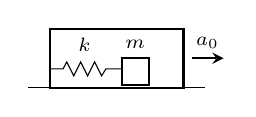
\begin{tikzpicture}[scale=0.68, baseline=(current bounding box.north)]
        % 车厢与地面
        \draw (-0.3,0) -- (3.0,0);
        \draw[thick] (0.1,0) rectangle (2.6,1.1);
        % 弹簧
        \draw (0.1,0.35) -- (0.35,0.35) -- (0.42,0.48) -- (0.55,0.22) -- (0.68,0.48) -- (0.81,0.22) -- (0.94,0.48) -- (1.07,0.22) -- (1.15,0.35) -- (1.45,0.35);
        \node[above] at (0.75,0.5) {\scriptsize $k$};
        % 滑块 m
        \draw[thick] (1.45,0.05) rectangle (1.95,0.55);
        \node[above] at (1.7,0.55) {\scriptsize $m$};
        % 加速度 a0
        \draw[->, >=stealth, thick] (2.75,0.55) -- (3.35,0.55);
        \node[above] at (3.05,0.55) {\scriptsize $a_0$};
    \end{tikzpicture}
    \end{minipage}

    \item 两个同方向同频率的简谐振动曲线如图所示，则合振动的表达式为：\blank[4.5cm]。
    \begin{center}
    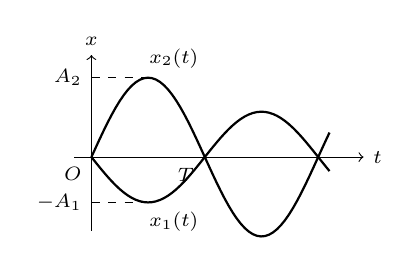
\begin{tikzpicture}[scale=0.72]
        \draw[->] (-0.3,0) -- (4.8,0) node[right] {\scriptsize $t$};
        \draw[->] (0,-1.3) -- (0,1.8) node[above] {\scriptsize $x$};
        \draw[thick, domain=0:4.2, samples=60] plot (\x, {-0.8*sin(90*\x)});
        \draw[thick, domain=0:4.2, samples=60] plot (\x, {1.4*sin(90*\x)});
        \draw[dashed] (0,1.4) node[left] {\scriptsize $A_2$} -- (1,1.4);
        \draw[dashed] (0,-0.8) node[left] {\scriptsize $-A_1$} -- (1,-0.8);
        \node[below left] at (0,0) {\scriptsize $O$};
        \node[below left] at (1.98,-0.02) {\scriptsize $T$};
        \node[above right] at (0.85,1.4) {\scriptsize $x_2(t)$};
        \node[below right] at (0.85,-0.8) {\scriptsize $x_1(t)$};
    \end{tikzpicture}
    \end{center}

    \item \begin{minipage}[t]{0.64\textwidth}
    如图所示，在竖直山坡左侧地面上有一辆警车以 $v_A = 10\ \mathrm{m/s}$ 的速度朝着山壁驶去，同时发出频率为 $\nu_0 = 1000\ \mathrm{Hz}$ 的警笛声。在警车左侧有一骑自行车者，他以速度 $v_B = 2\ \mathrm{m/s}$ 背向山壁离去。已知声波在空气中的传播速度为 $u=330\ \mathrm{m/s}$。骑自行车者接收到两列频率不同的声波，频率差为\blank[2.5cm]。
    \end{minipage}%
    \begin{minipage}[t]{0.34\textwidth}
    \centering
    \begin{tikzpicture}[scale=0.66, baseline=(current bounding box.north)]
        % 地面与山壁
        \draw[thick] (-0.3,0) -- (3.3,0) -- (3.3,1.3);
        \foreach \x in {-0.2,0.2,...,3.0} {\draw (\x,-0.15) -- (\x+0.15,0);}
        \foreach \y in {0.1,0.4,0.7,1.0} {\draw (3.3,\y) -- (3.45,\y+0.15);}
        % 骑车者 vB
        \fill (0.6,0.35) circle (2.2pt);
        \node[above] at (0.6,0.75) {\scriptsize 骑车者};
        \draw[<-, >=stealth] (0.15,0.55) -- (0.95,0.55);
        \node[left] at (0.15,0.55) {\scriptsize $v_B$};
        % 警车 vA
        \fill (2.0,0.35) circle (2.2pt);
        \node[above] at (2.0,0.75) {\scriptsize 警车};
        \draw[->, >=stealth] (1.65,0.55) -- (2.35,0.55);
        \node[right] at (2.35,0.55) {\scriptsize $v_A$};
    \end{tikzpicture}
    \end{minipage}

    \item 设入射波的表达式为 $y_1 = A\cos\left[2\pi\left(\nu t + \frac{x}{\lambda}\right) + \pi\right]$，波在 $x=0$ 处发生反射，反射点为固定端，则入射波和反射波合成驻波的波节坐标为\blank[3.5cm]。

    \item \begin{minipage}[t]{0.62\textwidth}
    在单缝夫琅禾费衍射示意图中，波长 $\lambda$ 的单色光垂直入射在单缝上，若对应于会聚在 $P$ 点的衍射光线在狭缝处的波阵面恰好分成 $4$ 个半波带，所画出的各条正入射光线间距相等。光线 $1$ 和 $3$ 在屏幕上 $P$ 点相遇时的相位差为\blank[2.0cm]。
    \end{minipage}%
    \begin{minipage}[t]{0.36\textwidth}
    \centering
    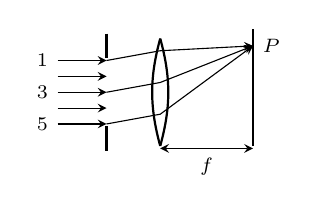
\begin{tikzpicture}[scale=0.62, baseline=(current bounding box.north)]
        % 单缝
        \draw[very thick] (0,1.2) -- (0,0.7);
        \draw[very thick] (0,-0.7) -- (0,-1.2);
        % 5条正入射光线 (1..5)
        \foreach \y in {0.65, 0.325, 0, -0.325, -0.65} {
            \draw[->, >=stealth] (-1.0,\y) -- (0,\y);
        }
        \node[left] at (-1.0,0.65) {\scriptsize $1$};
        \node[left] at (-1.0,0) {\scriptsize $3$};
        \node[left] at (-1.0,-0.65) {\scriptsize $5$};
        % 透镜
        \draw[thick] (1.1,-1.1) .. controls (1.32,-0.3) and (1.32,0.3) .. (1.1,1.1);
        \draw[thick] (1.1,-1.1) .. controls (0.88,-0.3) and (0.88,0.3) .. (1.1,1.1);
        % 屏幕
        \draw[thick] (3.0,-1.1) -- (3.0,1.3);
        \draw[<->, >=stealth, thin] (1.1,-1.15) -- (3.0,-1.15) node[midway, below] {\scriptsize $f$};
        % 衍射光线到 P
        \draw[->, >=stealth] (0,0.65) -- (1.1,0.85) -- (3.0,0.95) node[right] {\scriptsize $P$};
        \draw[->, >=stealth] (0,0) -- (1.1,0.2) -- (3.0,0.95);
        \draw[->, >=stealth] (0,-0.65) -- (1.1,-0.45) -- (3.0,0.95);
    \end{tikzpicture}
    \end{minipage}

    \item 设白天人的眼瞳直径为 $3\ \mathrm{mm}$，入射光波长为 $550\ \mathrm{nm}$，窗纱上两根细丝之间的距离为 $3\ \mathrm{mm}$，人眼睛可以距离窗纱\blank[2.2cm]$\mathrm{m}$ 时，恰能分辨。

    \item 用一束自然光从真空入射介质表面，当反射光为线偏振光时，测得此时折射光的折射角为 $30^\circ$，则介质的折射率为\blank[2.2cm]。

    \item 已知地球与金星的大小差不多，金星的平均温度约为 $773\ \mathrm{K}$，地球的平均温度约为 $293\ \mathrm{K}$。若把它们看作是理想黑体，在相同时间内金星与地球向空间辐射的能量之比大约为\blank[2.2cm]。

    \item 可用光电效应测定普朗克常数。如先后分别用波长 $\lambda_1$ 和 $\lambda_2$ 做光电效应实验，相应测得其遏止电势差为 $U_1$ 和 $U_2$，则可算得普朗克常数\blank[4.0cm]。

    \item \begin{minipage}[t]{0.68\textwidth}
    如图所示，频率为 $\nu$ 的入射光子与静止的自由电子发生碰撞和散射。如果散射光子的频率为 $\nu'$，反冲电子的动量为 $\vect{p}$，则在光子入射方向上的动量守恒的分量式为\blank[4.5cm]。
    \end{minipage}%
    \begin{minipage}[t]{0.30\textwidth}
    \centering
    \begin{tikzpicture}[scale=0.68, baseline=(current bounding box.north)]
        \draw[->, >=stealth, thick] (-1.4,0) -- (0,0) node[midway, above] {\scriptsize $\nu$};
        \draw[dashed] (0,0) -- (1.6,0);
        \draw[->, >=stealth, thick] (0,0) -- (40:1.4) node[above] {\scriptsize $\nu'$};
        \draw[->, >=stealth, thick] (0,0) -- (-42:1.4) node[below] {\scriptsize $e\text{ 反冲电子}$};
        \draw (0.55,0) arc (0:40:0.55);
        \node at (0.78,0.25) {\scriptsize $\phi$};
        \draw (0.5,0) arc (0:-42:0.5);
        \node at (0.72,-0.25) {\scriptsize $\theta$};
    \end{tikzpicture}
    \end{minipage}
\end{enumerate}

\section*{三、计算题（共 34 分）}

\begin{enumerate}[leftmargin=2em, itemsep=8pt, start=23]
    \item （10 分）如图所示为一平面简谐波在 $t=0$ 时刻的波形图，波的振幅为 $A$，设此简谐波的频率为 $250\ \mathrm{Hz}$，且此时质点 $P$ 的运动方向向下，原点处质点的位移为 $\frac{\sqrt{2}}{2}A$，求：\\
    （1）该波的波函数；\\
    （2）$x=100\ \mathrm{m}$ 处质点的振动表达式与振动速度表达式；\\
    （3）在波的传播方向上距原点分别为 $x_1 = 50\ \mathrm{m}$ 和 $x_2 = 200\ \mathrm{m}$ 两点间的相位差。
    \begin{center}
    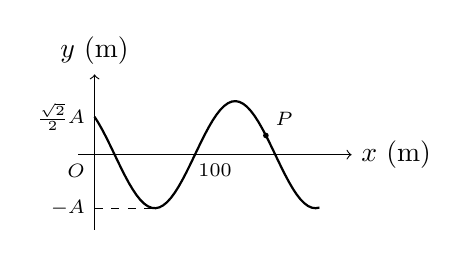
\begin{tikzpicture}[scale=0.68]
        \draw[->] (-0.3,0) -- (4.8,0) node[right] {$x\ (\mathrm{m})$};
        \draw[->] (0,-1.4) -- (0,1.5) node[above] {$y\ (\mathrm{m})$};
        \draw[thick, domain=0:4.2, samples=60] plot (\x, {cos(120*\x + 45)});
        \node[left] at (0,0.707) {\scriptsize $\frac{\sqrt{2}}{2}A$};
        \node[left] at (0,-1) {\scriptsize $-A$};
        \draw[dashed] (0,-1) -- (1.125,-1);
        \node[below left] at (0,0) {\scriptsize $O$};
        \fill (3.2,{cos(120*3.2+45)}) circle (1.5pt) node[above right] {\scriptsize $P$};
        \node[below] at (2.25,0) {\scriptsize $100$};
    \end{tikzpicture}
    \end{center}

    \item \begin{minipage}[t]{0.68\textwidth}
    （6 分）在图示的双缝干涉实验中，若用薄玻璃片（折射率 $n_1=1.4$）覆盖缝 $S_1$，用同样厚度的玻璃片（但折射率 $n_2=1.7$）覆盖缝 $S_2$，将使原来未放玻璃时屏上的中央明条纹处 $O$ 变为第五级明纹。设单色光波长 $\lambda=480\ \mathrm{nm}$，求玻璃片的厚度 $d$（可认为光线垂直穿过玻璃片）。
    \end{minipage}%
    \begin{minipage}[t]{0.30\textwidth}
    \centering
    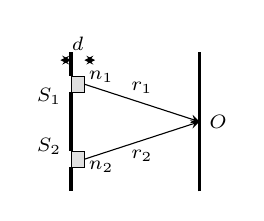
\begin{tikzpicture}[scale=0.68, baseline=(current bounding box.north)]
        \draw[very thick] (0,1.3) -- (0,0.85);
        \draw[very thick] (0,0.55) -- (0,-0.55);
        \draw[very thick] (0,-0.85) -- (0,-1.3);
        \draw[fill=gray!25] (0,0.55) rectangle (0.25,0.85);
        \draw[fill=gray!25] (0,-0.85) rectangle (0.25,-0.55);
        \node[below left] at (0,0.8) {\scriptsize $S_1$};
        \node[above left] at (0,-0.8) {\scriptsize $S_2$};
        \node[above right] at (0.15,0.55) {\scriptsize $n_1$};
        \node[below right] at (0.15,-0.55) {\scriptsize $n_2$};
        \draw[<->, >=stealth, thin] (-0.2,1.15) -- (0,1.15);
        \draw[<->, >=stealth, thin] (0.45,1.15) -- (0.25,1.15);
        \node[above] at (0.125,1.15) {\scriptsize $d$};
        \draw[thick] (2.4,-1.3) -- (2.4,1.3);
        \draw[->, >=stealth] (0.25,0.7) -- (2.4,0) node[midway, above] {\scriptsize $r_1$};
        \draw[->, >=stealth] (0.25,-0.7) -- (2.4,0) node[midway, below] {\scriptsize $r_2$};
        \node[right] at (2.4,0) {\scriptsize $O$};
    \end{tikzpicture}
    \end{minipage}

    \item \begin{minipage}[t]{0.62\textwidth}
    （9 分）如图所示，牛顿环装置的平凸透镜与平板玻璃有一小缝隙 $e_0$，透镜与平板玻璃间填充折射率为 $n$ 的透明液体，现用波长为 $\lambda$ 的单色光垂直照射，已知平凸透镜的曲率半径为 $R$。\\
    （1）求反射光形成的牛顿环的各级暗环半径；\\
    （2）证明：暗环的分布特征为内疏外密（即靠近中心的环间距大，越靠外侧的环间距越小）。
    \end{minipage}%
    \begin{minipage}[t]{0.36\textwidth}
    \centering
    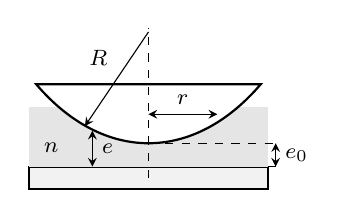
\begin{tikzpicture}[scale=0.95, baseline=(current bounding box.north)]
        % 平板玻璃
        \draw[thick, fill=gray!10] (-1.6,-0.5) rectangle (1.6,-0.2);
        % 透明液体 n
        \fill[gray!20] (-1.6,-0.2) rectangle (1.6,0.6);
        \node at (-1.3,0.05) {\footnotesize $n$};
        % 平凸透镜 (底部最低点 y=0.1125)
        \draw[thick, fill=white] (-1.5,0.9) -- (1.5,0.9) .. controls (0.6,-0.15) and (-0.6,-0.15) .. (-1.5,0.9) -- cycle;
        % 中心轴
        \draw[dashed] (0,-0.35) -- (0,1.65);
        % 缝隙 e0 标在右侧外延线上
        \draw[dashed, thin] (0,0.1125) -- (1.75,0.1125);
        \draw[dashed, thin] (1.6,-0.2) -- (1.75,-0.2);
        \draw[<->, >=stealth, thin] (1.7,-0.2) -- (1.7,0.1125) node[midway, right] {\footnotesize $e_0$};
        % 半径 r (向右，不与 R 交叉)
        \draw[<->, >=stealth, thin] (0,0.5) -- (0.92,0.5) node[midway, above] {\footnotesize $r$};
        % 厚度 e (左侧液层)
        \draw[<->, >=stealth, thin] (-0.75,-0.2) -- (-0.75,0.28) node[midway, right] {\footnotesize $e$};
        % 曲率半径 R (向左上方引出，完全避开 r)
        \draw[->, >=stealth, thin] (0,1.6) -- (-0.85,0.34);
        \node[above left] at (-0.42,1.02) {\footnotesize $R$};
    \end{tikzpicture}
    \end{minipage}

    \item （9 分）光栅衍射实验中将波长 $\lambda = 540\ \mathrm{nm}$ 的光垂直照射在光栅上，衍射光强分布如图所示，$\theta$ 为衍射角，$\sin\theta = 0.30$ 及 $\sin\theta = 0.60$ 时有主极大缺级，$\theta = \arcsin 0.3$ 对应于单缝衍射中央明纹的边界，且两主明纹间有 $5$ 个暗纹，则光栅的狭缝总数 $N$、光栅常数 $d$ 以及狭缝宽度 $a$ 分别为多少？最多能观察到哪些级数的条纹？
    \begin{center}
    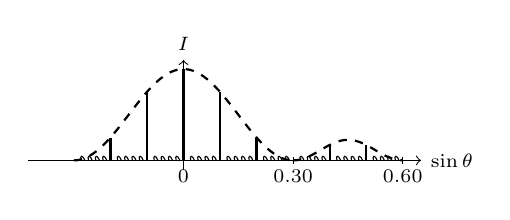
\begin{tikzpicture}[scale=0.58]
        \draw[->] (-3.4,0) -- (5.2,0) node[right] {\scriptsize $\sin\theta$};
        \draw[->] (0,-0.2) -- (0,2.2) node[above] {\scriptsize $I$};
        \node[below] at (0,0) {\scriptsize $0$};
        \node[below] at (2.4,0) {\scriptsize $0.30$};
        \node[below] at (4.8,0) {\scriptsize $0.60$};
        % 单缝衍射包络 (虚线)
        \draw[dashed, thick, domain=-2.4:2.4, samples=60] plot (\x, {2.0*(cos(90*\x/2.4))^2});
        \draw[dashed, thick, domain=2.4:4.8, samples=40] plot (\x, {0.45*(sin(180*(\x-2.4)/2.4))^2});
        % 主极大峰 (k=0 at 0; k=+-1 at +-0.8; k=+-2 at +-1.6; k=3 missing at 2.4; k=4 at 3.2; k=5 at 4.0; k=6 missing at 4.8)
        \draw[thick] (0,0) -- (0,2.0);
        \draw[thick] (-0.8,0) -- (-0.8,1.5);
        \draw[thick] (0.8,0) -- (0.8,1.5);
        \draw[thick] (-1.6,0) -- (-1.6,0.5);
        \draw[thick] (1.6,0) -- (1.6,0.5);
        \draw[thick] (3.2,0) -- (3.2,0.34);
        \draw[thick] (4.0,0) -- (4.0,0.34);
        % 缺级十字标记
        \draw (2.4,-0.08) -- (2.4,0.08);
        \draw (4.8,-0.08) -- (4.8,0.08);
        % 次极大示意 (两主明纹间 4 个小次极大 => 5 个暗纹)
        \foreach \a in {-2.4,-1.6,-0.8,0,0.8,1.6,2.4,3.2,4.0} {
            \foreach \j in {1,2,3,4} {
                \draw[thin] ({\a + \j*0.16},0) .. controls ({\a + \j*0.16 - 0.04},0.12) and ({\a + \j*0.16 + 0.04},0.12) .. ({\a + \j*0.16 + 0.08},0);
            }
        }
    \end{tikzpicture}
    \end{center}
\end{enumerate}

\end{document}
